\documentclass[12pt]{exam}
\printanswers
\framedsolutions
\usepackage[utf8]{inputenc}
\usepackage[a4paper, total={6in, 4in}]{geometry}
\usepackage{geometry}
\usepackage{amsmath}
\usepackage{amssymb}
\usepackage{tikz}
\geometry{left=2cm, right=2cm, top=2cm, bottom=2cm}
\usetikzlibrary{automata, positioning, arrows}
\tikzset{
->, % makes the edges directed
>=stealth', % makes the arrow heads bold
node distance=3cm, % specifies the minimum distance between two nodes. Change if necessary.
every state/.style={thick}, % sets the properties for each ’state’ node
initial text=$ $, % sets the text that appears on the start arrow
}
\newcommand\scalemath[2]{\scalebox{#1}{\mbox{\ensuremath{\displaystyle #2}}}}

\title{
  Assignment 1\\
  \large CMPUT 474
}
\author{Pranav Wadhwa\\1629510}

\begin{document}
\maketitle
\noindent

\begin{questions}
  \question % Question 1
  How many finite automata are there? How many regular expressions are there? How many regular languages are there? (Give a separate answer for each)

  \begin{solution}

    Every finite automata can be described as a string. So the set of automatas are subsets of strings. There are uncountable infinite number of strings. So there are \emph{countable infinite} finite automata.

    Since there are countably infinite finite automata and each finite automata is decribed by a regular expresion then there are also \emph{countable infinite} regular expressions.

    Since each regular expression describles a regular language and each regular language has a regular expression then there are \emph{conutable infinite} regular languages.


  \end{solution}

  \question % question 2

  Give state diagrams for DFAs that recognize the following languages. Assume that alphabet is $\Sigma = \{0,1\}$ in each case.

  \begin{parts}
    \part Strings that begin with 1 and end with 10
    \part Strings that contain at least three occurrences of 11
    \part Strings without leading 0s
    \part Strings of length at most 4
    \part Strings containing 10 and 11
    \part Strings with length divisible by 4
  \end{parts}

  \begin{solution}

    \begin{parts}
      \part Strings that begin with 1 and end with 10\\
      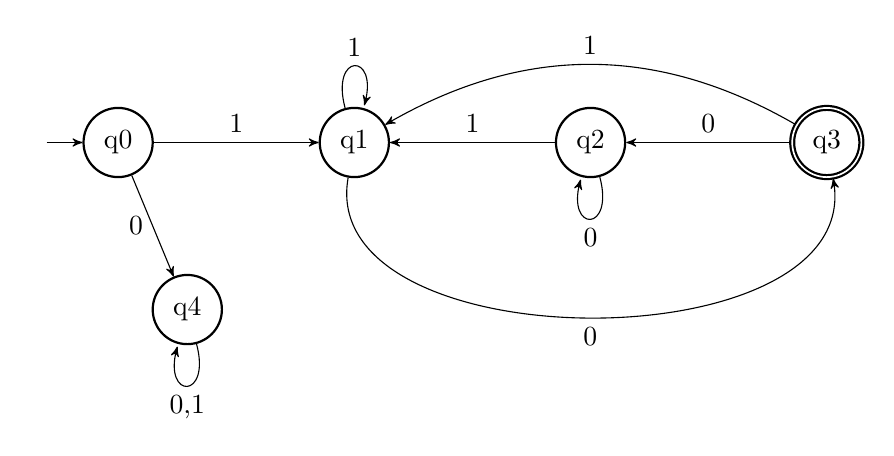
\begin{tikzpicture}
        \node[state, initial] (q0) {q0};
        \node[state, right of=q0] (q1) {q1};
        \node[state, right of=q1] (q2) {q2};
        \node[state, right of=q2, accepting] (q3) {q3};
        \node[state, below left of=q1] (q4) {q4};


        \draw (q0) edge[above] node{1} (q1)
        (q1) edge[bend right=100, below,] node{0} (q3)
        (q1) edge[loop above] node{1} (q1)
        (q3) edge[bend right, above] node{1} (q1)
        (q3) edge[above] node{0} (q2)
        (q2) edge[above] node{1} (q1)
        (q2) edge[loop below] node{0} (q2)
        (q0) edge[left] node{0} (q4)
        (q4) edge[loop below, below] node{0,1} (q4);
      \end{tikzpicture}


      \part Strings that contain at least three occurrences of 11\\
      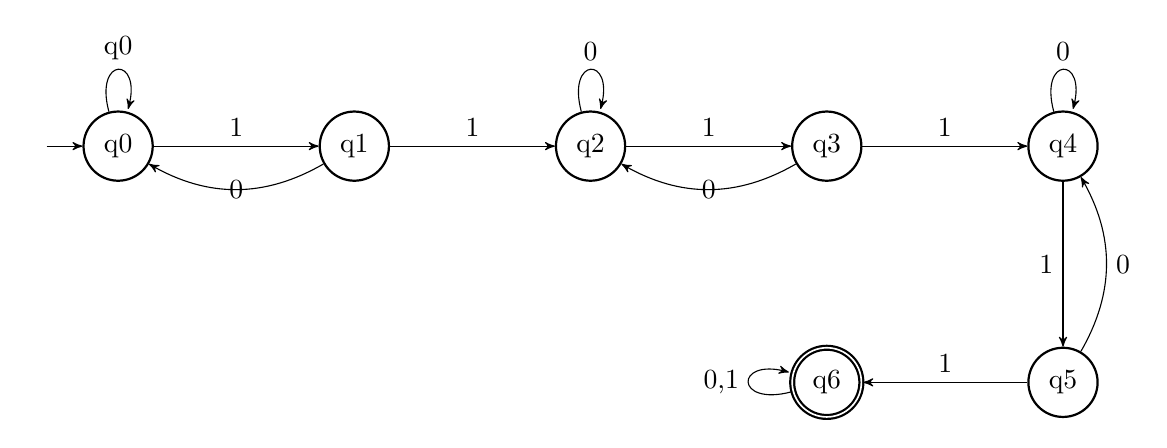
\begin{tikzpicture}
        \node[state, initial] (q0) {q0};
        \node[state, right of=q0] (q1) {q1};
        \node[state, right of=q1] (q2) {q2};
        \node[state, right of=q2] (q3) {q3};
        \node[state, right of=q3] (q4) {q4};
        \node[state, below of=q4] (q5) {q5};
        \node[state, accepting, left of=q5] (q6) {q6};

        \draw (q0) edge[loop above] node{q0} (q0)
        (q0) edge[above] node{1} (q1)
        (q1) edge[bend left] node{0} (q0)
        (q1) edge[above] node{1} (q2)
        (q2) edge[loop above] node{0} (q2)
        (q2) edge[above] node{1} (q3)
        (q3) edge[bend left] node{0} (q2)
        (q3) edge[above] node{1} (q4)
        (q4) edge[loop above] node{0} (q4)
        (q4) edge[left] node{1} (q5)
        (q5) edge[above] node{1} (q6)
        (q5) edge[bend right, right] node{0} (q4)
        (q6) edge[loop left] node{0,1} (q6);
      \end{tikzpicture}


      \part Strings without leading 0s\\

      \begin{tikzpicture}
        \node[state, initial] (q0) {q0};
        \node[state, accepting, right of=q0] (q2) {q2};
        \node[state, below left of=q2] (q3) {q3};

        \draw (q0) edge[above] node{1} (q1)
        (q2) edge[loop right] node{0,1} (q2)
        (q0) edge[left] node{0} (q3)
        (q3) edge[loop right] node{0,1} (q3);
      \end{tikzpicture}


      \part Strings of length at most 4\\

      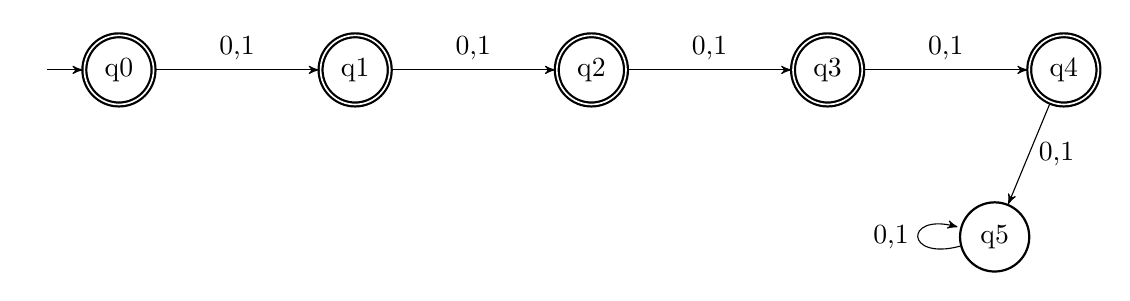
\begin{tikzpicture}
        \node[state, initial, accepting] (q0) {q0};
        \node[state, accepting, right of=q0] (q1) {q1};
        \node[state, accepting, right of=q1] (q2) {q2};
        \node[state, accepting, right of=q2] (q3) {q3};
        \node[state, accepting, right of=q3] (q4) {q4};
        \node[state, below right of=q3] (q5) {q5};


        \draw (q0) edge[above] node{0,1} (q1)
        (q1) edge[above] node{0,1} (q2)
        (q2) edge[above] node{0,1} (q3)
        (q3) edge[above] node{0,1} (q4)
        (q4) edge[right] node{0,1} (q5)
        (q5) edge[loop left] node{0,1} (q5);
      \end{tikzpicture}

      \part Strings containing 10 and 11\\

      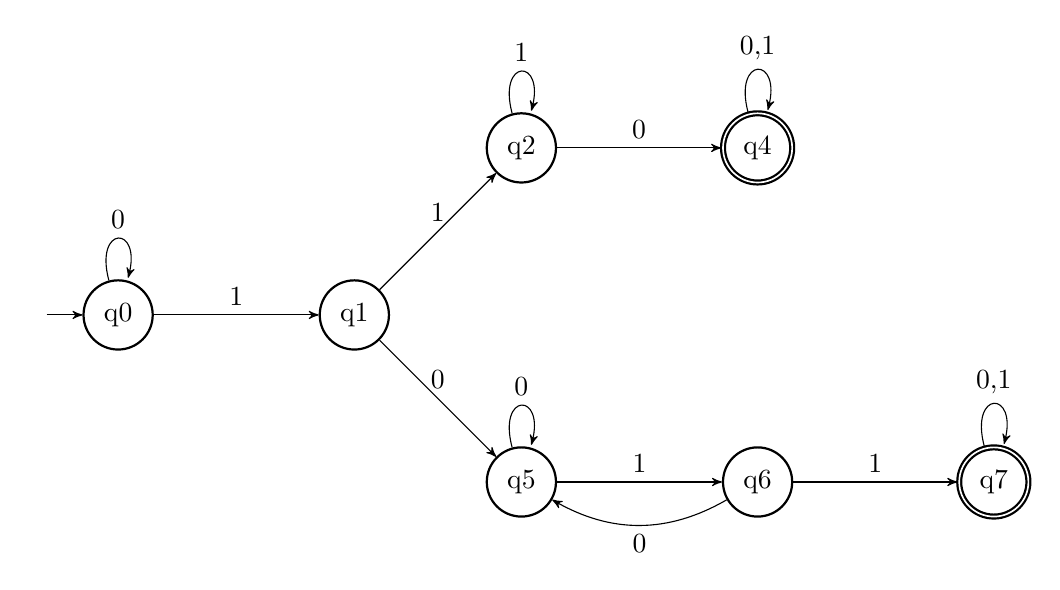
\begin{tikzpicture}
        \node[state, initial] (0) {q0};
        \node[state, right of=0] (1) {q1};
        \node[state, above right of=1] (2) {q2};
        \node[state, accepting,right of=2] (4) {q4};
        \node[state, below right of=1] (5) {q5};
        \node[state, right of=5] (6) {q6};
        \node[state, accepting, right of=6] (7) {q7};


        \draw (0) edge[loop above] node{0} (0)
        (0) edge[above] node{1} (1)
        (1) edge[above] node{1} (2)
        (1) edge[above] node{0} (5)
        (2) edge[above] node{0} (4)
        (2) edge[loop above] node{1} (2)
        (4) edge[loop above] node{0,1} (4)
        (5) edge[loop above] node{0} (5)
        (5) edge[above] node{1} (6)
        (6) edge[bend left, below] node{0} (5)
        (6) edge[above] node{1} (7)
        (7) edge[loop above] node{0,1} (7);
      \end{tikzpicture}

      \part Strings with length divisible by 4\\

      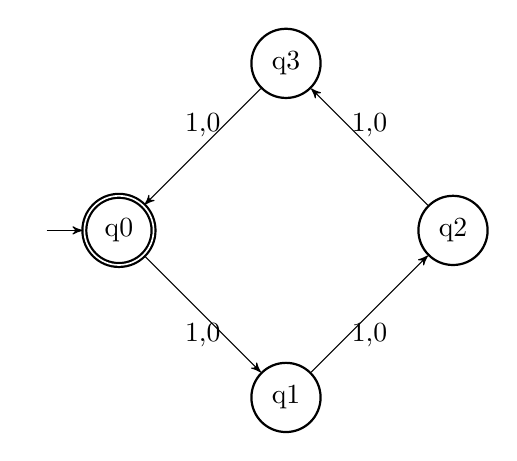
\begin{tikzpicture}
        \node[state, initial, accepting] (q0) {q0};
        \node[state, below right of=q0] (q1) {q1};
        \node[state, above right of=q1] (q2) {q2};
        \node[state, above left of=q2] (q3) {q3};


        \draw (q0) edge[below] node{1,0} (q1)
        (q1) edge[below] node{1,0} (q2)
        (q2) edge[above] node{1,0} (q3)
        (q3) edge[above] node{1,0} (q0);
      \end{tikzpicture}

    \end{parts}



  \end{solution}

  \question % Question 3
  For each of the following NFAs, draw a DFA that accepts the same language.

  \begin{parts}
    \part % part a
      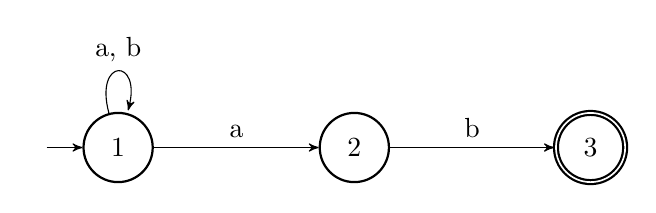
\begin{tikzpicture}
        \node[state, initial] (q1) {1};
        \node[state, right of=q1] (q2) {2};
        \node[state, accepting, right of=q2] (q3) {3};

        \draw (q1) edge[loop above] node{a, b} (q1)
        (q1) edge[above] node{a} (q2)
        (q2) edge[above] node{b} (q3);
      \end{tikzpicture}

    \part % part b
      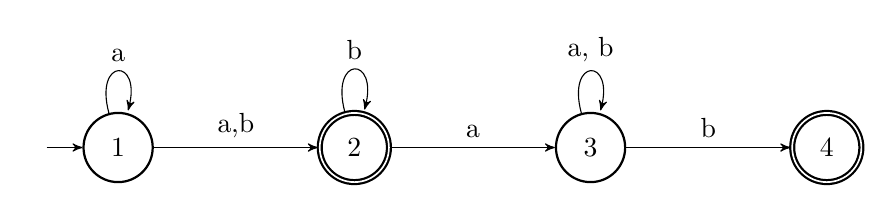
\begin{tikzpicture}
        \node[state, initial] (q1) {1};
        \node[state, accepting, right of=q1] (q2) {2};
        \node[state, right of=q2] (q3) {3};
        \node[state, accepting, right of=q3] (q4) {4};

        \draw (q1) edge[loop above] node{a} (q1)
        (q1) edge[above] node{a,b} (q2)
        (q2) edge[loop above] node{b} (q2)
        (q2) edge[above] node{a} (q3)
        (q3) edge[above] node{b} (q4)
        (q3) edge[loop above] node{a, b} (q3);
      \end{tikzpicture}

    \part % part c
      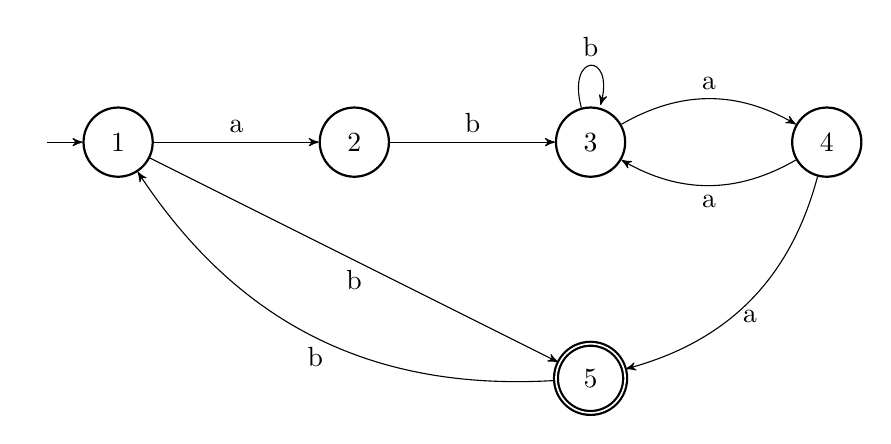
\begin{tikzpicture}
        \node[state, initial] (q1) {1};
        \node[state, right of=q1] (q2) {2};
        \node[state, right of=q2] (q3) {3};
        \node[state, right of=q3] (q4) {4};
        \node[state, accepting, below of=q3] (q5) {5};

        \draw (q1) edge[above] node{a} (q2)
        (q2) edge[above] node{b} (q3)
        (q3) edge[loop above] node{b} (q3)
        (q3) edge[bend left, above] node{a} (q4)
        (q4) edge[bend left, below] node{a} (q3)
        (q1) edge[below] node{b} (q5)
        (q5) edge[bend left, below] node{b} (q1)
        (q4) edge[bend left, below] node{a} (q5);
      \end{tikzpicture}

    \part % part d
      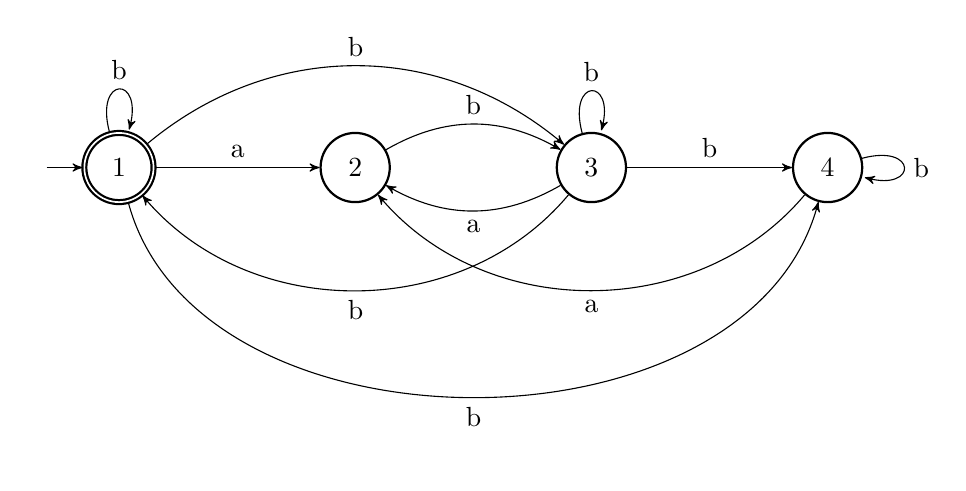
\begin{tikzpicture}
        \node[state, initial, accepting] (q1) {1};
        \node[state, right of=q1] (2) {2};
        \node[state, right of=2] (3) {3};
        \node[state, right of=3] (4) {4};

        \draw (q1) edge[loop above] node{b} (q1)
        (q1) edge[above] node{a} (2)
        (q1) edge[bend left=40, above] node{b} (3)
        (q1) edge[bend right=75, below] node{b} (4)
        (2) edge[bend left, above] node{b} (3)
        (3) edge[bend left, below] node{a} (2)
        (3) edge[bend left=50, below] node{b} (q1)
        (3) edge[loop above] node{b} (3)
        (3) edge[above] node{b} (4)
        (4) edge[loop right] node{b} (4)
        (4) edge[bend left=50, below] node{a} (2);
      \end{tikzpicture}
  \end{parts}


  \begin{solution}


    \begin{parts}

      \part DFA for part a)\\

      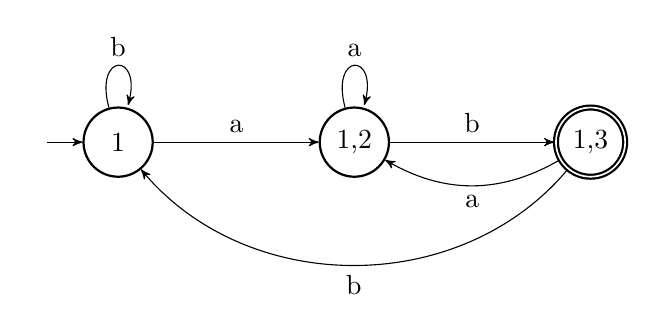
\begin{tikzpicture}
        \node[state, initial] (1) {1};
        \node[state, right of=1] (12) {1,2};
        \node[state, accepting, right of=12] (13) {1,3};


        \draw (1) edge[loop above] node{b} (1)
        (1) edge[above] node{a} (12)
        (12) edge[loop above] node{a} (12)
        (12) edge[above] node{b} (13)
        (13) edge[bend left, below] node{a} (12)
        (13) edge[bend left=50, below] node{b} (1);
      \end{tikzpicture}

      \part DFA for part b)\\

      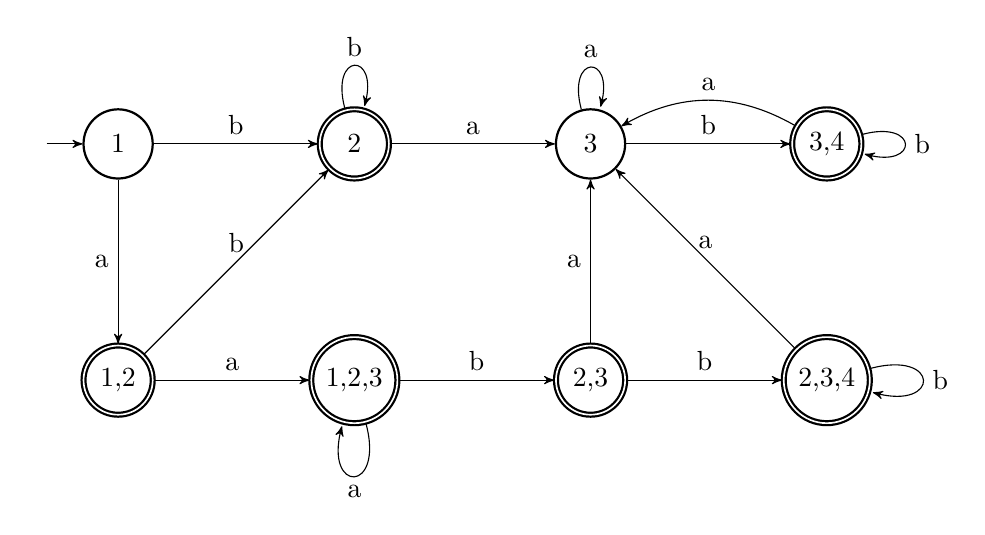
\begin{tikzpicture}
        \node[state, initial] (1) {1};
        \node[state, accepting, right of=1] (2) {2};
        \node[state, right of=2] (3) {3};
        \node[state, accepting, right of=3] (34) {3,4};
        \node[state, accepting, below of=1] (12) {1,2};
        \node[state, accepting, right of=12] (123) {1,2,3};
        \node[state, accepting, right of=123] (23) {2,3};
        \node[state, accepting, right of=23] (234) {2,3,4};


        \draw (1) edge[above] node{b} (2)
        (1) edge[left] node{a} (12)
        (2) edge[loop above] node{b} (2)
        (2) edge[above] node{a} (3)
        (3) edge[loop above] node{a} (3)
        (3) edge[above] node{b} (34)
        (34) edge[bend right, above] node{a} (3)
        (34) edge[loop right] node{b} (34)
        (12) edge[above] node{b} (2)
        (12) edge[above] node{a} (123)
        (123) edge[loop below] node{a} (123)
        (123) edge[above] node{b} (23)
        (23) edge[left] node{a} (3)
        (23) edge[above] node{b} (234)
        (234) edge[above] node{a} (3)
        (234) edge[loop right] node{b} (234);
      \end{tikzpicture}



      \part DFA for part c)\\

      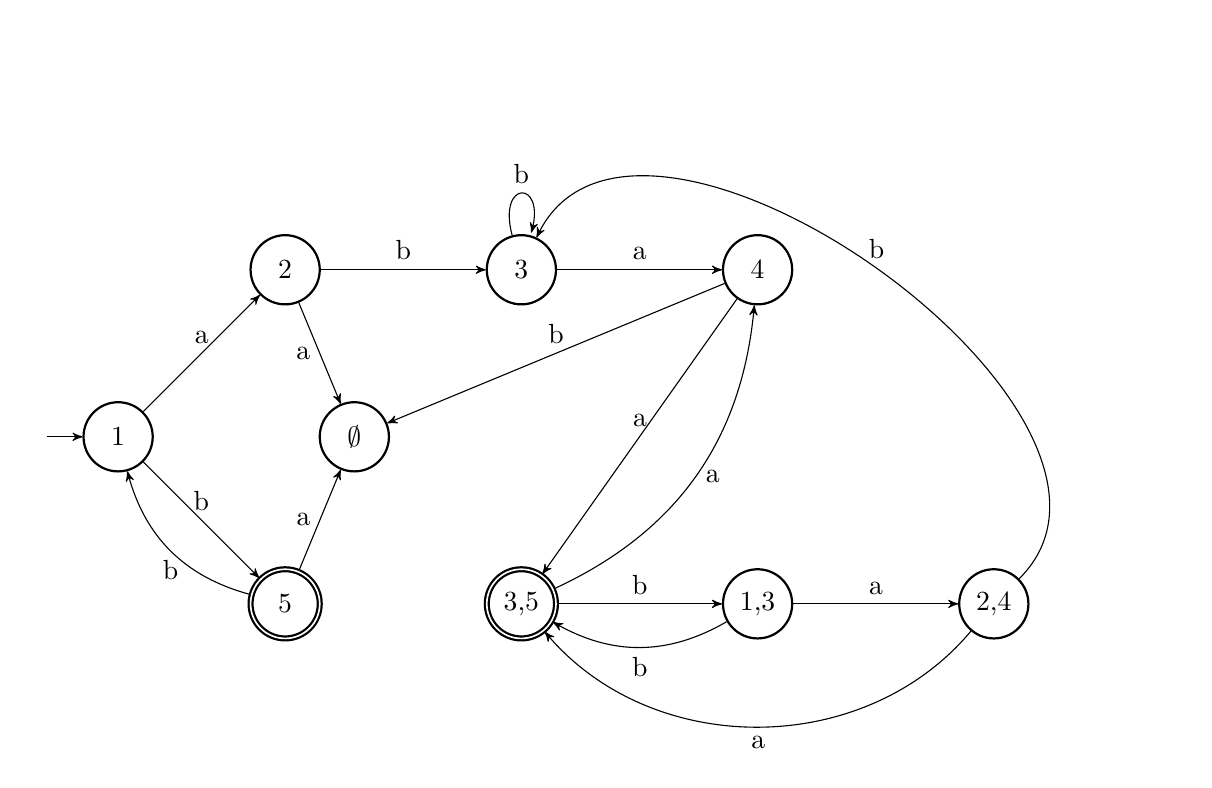
\begin{tikzpicture}
        \node[state, initial] (1) {1};
        \node[state, above right of=1] (2) {2};
        \node[state, right of=2] (3) {3};
        \node[state, right of=3] (4) {4};
        \node[state, accepting, below right of=1] (5) {5};
        \node[state, accepting,right of=5] (35) {3,5};
        \node[state, right of=35] (13) {1,3};
        \node[state, right of=13] (24) {2,4};
        \node[state, right of=1] (emp) {$\emptyset$};

        \draw (1) edge[above] node{a} (2)
        (1) edge[above] node{b} (5)
        (2) edge[above] node{b} (3)
        (3) edge[above] node{a} (4)
        (3) edge[loop above] node{b} (3)
        (4) edge[above] node{a} (35)
        (5) edge[bend left, below] node{b} (1)
        (35) edge[bend right, right] node{a} (4)
        (35) edge[above] node{b} (13)
        (13) edge[above] node{a} (24)
        (13) edge[bend left, below] node{b} (35)
        (24) edge[bend left=50, below] node{a} (35)
        (24) edge[bend right=100, above] node{b} (3)
        (2) edge[left] node{a} (emp)
        (5) edge[left] node{a} (emp)
        (4) edge[above] node{b} (emp);
      \end{tikzpicture}

      \part DFA for part d)\\

      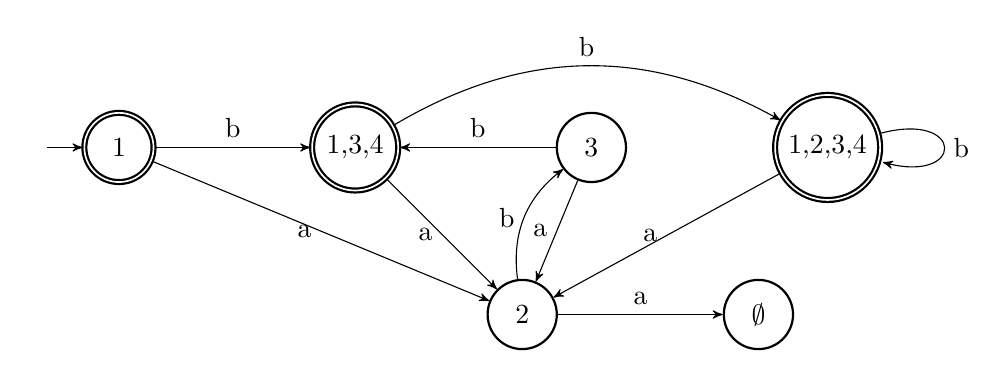
\begin{tikzpicture}
        \node[state, accepting, initial] (1) {1};
        \node[state, accepting, right of=1] (134) {1,3,4};
        \node[state, right of=134] (3) {3};
        \node[state, accepting, right of=3] (1234) {1,2,3,4};
        \node[state, below right of=134] (2) {2};
        \node[state, right of=2] (e) {$\emptyset$};

        \draw (1) edge[left] node{a} (2)
        (1) edge[above] node{b} (134)
        (2) edge[above] node{a} (e)
        (2) edge[bend left, left] node{b} (3)
        (134) edge[left] node{a} (2)
        (134) edge[bend left, above] node{b} (1234)
        (3) edge[left] node{a} (2)
        (3) edge[above] node{b} (134)
        (1234) edge[left] node{a} (2)
        (1234) edge[loop right] node{b} (1234);
      \end{tikzpicture}

    \end{parts}

  \end{solution}


\question
Let the alphabet be $\Sigma = \{0,1\}$. Write a regular expression for the language consisting of strings that do not contain $101$. Prove your claim.


\begin{solution}

  \emph{Idea}: To write an regular expression that does not contain the string $101$, every 1 need to be followed by 2 $0$s.\\
  \emph{Sol}:\\
  The regular expression that does not contain the string $101$
  \[0^{*}(1^{*}00^{*})^{*}1^{*}0^{*}\]

  \emph{Proof}:
  We can create a DFA that recognizes this expression.

  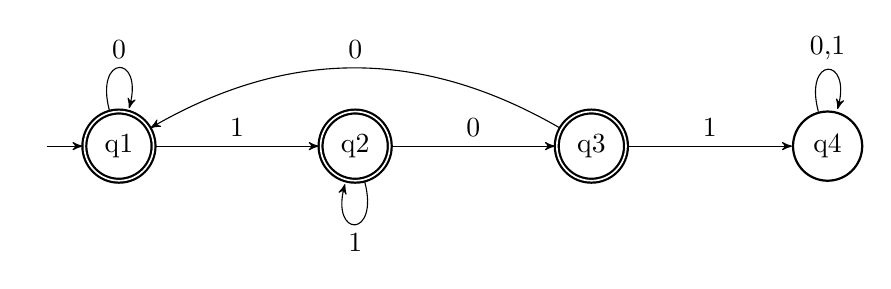
\begin{tikzpicture}
    \node[state, accepting,initial] (1) {q1};
    \node[state, accepting, right of=1] (2) {q2};
    \node[state, accepting, right of=2] (3) {q3};
    \node[state, right of=3] (4) {q4};


    \draw (1) edge[loop above] node{0} (1)
    (1) edge[above] node{1} (2)
    (2) edge[loop below] node{1} (2)
    (2) edge[above] node{0} (3)
    (3) edge[bend right, above] node{0} (1)
    (3) edge[above] node{1} (4)
    (4) edge[loop above] node{0,1} (4);

  \end{tikzpicture}

\end{solution}

\question % Question 5
Let the alphabet be $\Sigma = \{0,1,+, =\}$ and consider the language
\[ADD = \{x = y+z | x,y,z \text{ are binary integers and } x \text{ is the sum of } y \text{ and } z\}\]
Show that $ADD$ is not regular.

\begin{solution}

  \emph{Idea}: We see that the language can only contain one of $=$, $+$ each. We will use this condition to form some form of a binary equation that makes the equation incorrect.\\

  \emph{Proof}:
  Let $ADD$ be the language
  \[ADD = \{x = y+z | x,y,z \text{ are binary integers and } x \text{ is the sum of } y \text{ and } z\}\]
  We use the pumping lemma to prove $ADD$ is not regular. The proof is by contradiction.

  Assume to the contrary that $ADD$ is regular. Let $p$ be the length given by the pumping lemma. We choose $s = 1^{p+1}=10^{p}+1^{p}$ to be a string and $s$ is a member of $ADD$. As $s$ is a member of $ADD$, $|s| \geq p$  so the pumping lemma guarantees that $s$ can be split into $s=xyz$, where for any $i \geq 0$ the string $xy^{i}z$ is in $ADD$.


  Now we observe in $s$ that the first $p$ are all before the $=$ sign then $y$ must consists of all $1$ s. We know through the pumping lemma that $x$ and $z$ can be $\epsilon$. So we take $x=\epsilon$ and take $i=0$. Then $s\notin ADD$, as that expression in not an equation at all as there is nothing before the $=$ sign.

  Another way to prove it would be to look at the string $s = xz$. Here the left hand side and the right hand sign of the equation would not be equal, making the equation not true.

  Thus, there is a contradiction and $ADD$ is not regular.
\end{solution}


\question % question 6
Let
\[\scalemath{1.1}{ \Sigma_{3} = \{
  \begin{bmatrix}
    0\\
    0\\
    0
  \end{bmatrix}
  ,
  \begin{bmatrix}
    0\\
    0\\
    1
  \end{bmatrix}
  ,
  \begin{bmatrix}
    0\\
    1\\
    0
  \end{bmatrix}
  , \ldots,
  \begin{bmatrix}
    1\\
    1\\
    1
  \end{bmatrix}
  \}}\]
That is, $\Sigma_{3}$ contains all $3$ columns of $0s$ and $1s$. A string of symbols in $\Sigma_{3}$ goves three rows of $0s$ and $1s$. Consider each row to be a bianry number \emph{ordered from the least signifcant bits on the left to the most signifcant bits on the right} (that is, reversed from the normal convention). Let

\[\scalemath{1.10}{B = \{w \in \Sigma_{3}^{*}| \text{ the bottom row of } w \text{ is the sum of the top two rows} \} }\]
For example,

\[ \scalemath{1.10}{\begin{bmatrix}
    1\\
    1\\
    0
  \end{bmatrix}
  \begin{bmatrix}
    1\\
    0\\
    0
  \end{bmatrix}
  \begin{bmatrix}
    0\\
    0\\
    1
  \end{bmatrix}
  \in B, \text{but}
  \begin{bmatrix}
    1\\
    0\\
    1
  \end{bmatrix}
  \begin{bmatrix}
    0\\
    0\\
    1
  \end{bmatrix}
  \notin B.
}\]
Show that $B$ is regular.

\begin{solution}

  To show that $B$ is regular we can draw a NFA that recognizes $B$.

  \emph{Idea}: Since the alphabet only recognizes columns $0$s and $1$s. We will have to keep count of the carry and take it over the next string. We can easily count it using states as the carry over bit can only be $0$ or $1$. So there will be 2 state $q_{0}$ and $q_{1}$ in the NFA which will only take a subset of strings from $\Sigma_{3}$ and rest would not be accepted.

  \emph{Proof}:
  Let $M$ be a NFA that recognizes $B$ such that $M = (Q,\Sigma_{r}, \delta, q_{0}, F)$.
  \begin{enumerate}
    \item{} $Q = \{q_{0}, q_{1}\}$
    \item{} $\Sigma_{3} =\{
    \begin{bmatrix}
      0\\
      0\\
      1\\
    \end{bmatrix}
    \begin{bmatrix}
      0\\
      0\\
      1
    \end{bmatrix}
    , \ldots,
    \begin{bmatrix}
      1\\
      1\\
      1\\
    \end{bmatrix}\}$
    \item{} Start State: $q_{0}$
    \item{} $F = q_{0}$
    \item{} $\delta$ is given by:

    $\delta(q_{0}, a) = q_{0}$ if $a = \begin{bmatrix}
      0\\
      0\\
      0
    \end{bmatrix},
    \begin{bmatrix}
      0\\
      1\\
      1
    \end{bmatrix},
    \begin{bmatrix}
      1\\
      0\\
      1
    \end{bmatrix}$

    $\delta(q_{0}, a) = q_{1}$ if $a = \begin{bmatrix}
      1\\
      1\\
      0
    \end{bmatrix}$

    $\delta(q_{q}, a) = q_{1}$ if $a = \begin{bmatrix}
      1\\
      0\\
      0
    \end{bmatrix},
    \begin{bmatrix}
      0\\
      1\\
      0
    \end{bmatrix},
    \begin{bmatrix}
      1\\
      1\\
      1
    \end{bmatrix}$

    $\delta(q_{1}, a) = q_{0}$ if $a = \begin{bmatrix}
      0\\
      0\\
      1
    \end{bmatrix}$
  \end{enumerate}

  Rest of the string not mentioned above would not be accepted by $M$.

  For example: We can see that the string $\begin{bmatrix}
    1\\
    0\\
    1
  \end{bmatrix} \begin{bmatrix}
    0\\
    0\\
    1
    \end{bmatrix}$ would not be accepted by $M$ as after accepting $\begin{bmatrix}1\\0\\1\end{bmatrix}$ the machine is is at state $q_{0}$. There is no transition state for $\begin{bmatrix}0\\0\\1\end{bmatrix}$ from $q_{0}$ so the string is not accepted.

\end{solution}




\question % question 7
Suppost $A$ is a regular language. Show that the language
\[B = \{x | \text{there is some } y \text{ such that } |x| = |y| \text{ and } xy \in A \}\]
is also regular.

\begin{solution}

  \emph{Idea}: Since $xy$ is a concatenation of 2 strings. We can use the proof of clousure under concatenation.

  \emph{Proof}: Assume that $A$ is a regular language and $B = \{x|{} \text{there is some }y \text{ such that } |x| = |y| \text{ and } xy\in A\}$. Let $xy$ be a string such that $xy\in A$, $|x|=|y|$ and $x\in B$. We want to show that $B$ is regular.


  Lets assume that $B$ is not a regular language. Under the proof of closure any expression $R = R_{1} \circ R_{2}$ where $R_{1} \text{and } R_{2}$ are regular expression would result in a regular expression $R$. Since $B$ is not regular then $x$ is not a regular expression. But $x\circ y\in A$ which is a regular language. This is a contradiction under closure of concatenation. Hence $B$ is also regular.


\end{solution}



\question % question 8
\begin{parts}
  \part Let $A = \{1^{k}y | y\in \{0,1\}^{*} \text{ and } y \text{ contains at least } k\text{ } 1s, \text{for } k\geq 1\}$. Show that $A$ is regular.

  \part Let $B = \{1^{k}y | y\in \{0,1\}^{*} \text{ and } y \text{ contains at most } k\text{ }1s, \text{for } k\geq 1 \}$/ Show that $B$ is not regular.
\end{parts}


\begin{solution}

  \begin{parts}


    \part{}
    \emph{Idea}: Since the question doesn't restrict the value of $k$ we can set $k=1$. This means that every string should start with $1$ and then concatenate $1y$ so that the restriction is fulfilled.

    A regular expression describing $A$:
    \[10^{*}1\{0,1\}^{*}\]

    A DFA describing the regular expression.

    \begin{tikzpicture}
      \node[state, initial] (0) {q0};
      \node[state, right of=1] (1) {q2};
      \node[state, right of=3] (2) {q3};


      \draw (0) edge[above] node{1} (1)
      (1) edge[above] node{1} (2)
      (1) edge[loop above] node{0} (1)
      (2) edge[loop right] node{0,1} (2);
    \end{tikzpicture}

    \part{} Let $B = \{1^{k}b | b\in \{0,1\}^{*} \text{ and } b \text{ contains at most } k\text{ }1s, \text{for } k\geq 1 \}$/ Show that $B$ is not regular.

    We will use the pumping lemma to show that $B$ is not regular.

    Assume the contrary that $B$ is regular. Let $p$ be the pumping lenth given by the pumping lemma. Let s be a string $s = 1^{p}01^{p}$ and $s\in B$. The lemma guarantees that s can be split into $s = xyz$, where for any $i\geq 0$ $xy^{i}z \in B$ and $|xy| \le p$. Clearly, $y$ contains the substring of $1^{p}$ to satify the condition. Let the $n=|y|$. The string $xz=1^{(p-n)}01^{p} = 1^{p-n}b$ where b contains $p$ $1s$. Since $p-n < p$ the string $xz$ is not in $B$ which is a contradiction. So $B$ is not regular.

    \end{parts}
\end{solution}


\question % question 9
Every regular expression specifies a regular language over string from a finite alphabet $\Sigma$. However, the set of regular expressions, itself is a language over strings from an expanded alphabet $\Sigma \cup \{\epsilon, \emptyset, (,), \cup, \circ, *\}$. Is the set of regular expression a regular language. Explain your answer.


\begin{solution}
  Assume a $R_{1}$ and $R_{2}$ to be regular expression from the expanded alphabet $\Sigma \cup \{\epsilon, \emptyset, (,), \cup, \circ, *\}$. Take $\{R_{1}, R_{2}\}$ to be the set of these 2 regular expressions. Then this set would describle a regular language described by $R_{1}\cup R_{2}$.
\end{solution}


\question % question 10
Is there a \emph{universal} finite automation? That is, is there a single finite automaton, say $M$, such that given a string $s_{N}w$, where $s_{N}$ is a string that describes a finite automaton $N$ and $w$ is an input string, $M$ accepts $s_{N}w$ if and only if $N$ accepts $w$? Explain your answer.

\begin{solution}

  Assume that there is universal finite automation $M$ described by this 5-tuple $(Q,\Sigma, \delta, q_{0}, F)$ that takes a $s_{N}w$ where $s_{N}$ describes a finite automaton $N$ and $w$ is an input string that $N$ accepts. Here $N$ is described as $(Q_{N}, \Sigma_{N}, \delta_{N}, q_{N_{0}}, F_{n})$

  We know that there are countable infinite regular languages which has a countable infinite automaton. Lets assume that the finite automation $N$ has a total number of state $|Q_{N}| = n$
  Let's say that in the universal automaton $M$ there are $m$ set of state. So $|Q| = m $.
  For the universal automation to give the correct result it needs to have atleast $m \ge n$. Now assumne another finite automation $P$ which has number of state $|Q_{P}| = p > m+1$ and assume a string $s_{P}w_{P}$ where $s_{P}$ describes $P$ and $w_{p}$ is an input string.

 But M needs $|Q|\ge |Q_{p}|$ to accept the given string. This casues a contradiction. Therfore, $M$ is is not a universal finite automation.

\end{solution}



\end{questions}

\end{document}

